\section{Framework Concept}

\subsection{Introduction}

The Golem System is a framework for trading computing power in the Peer2Peer (P2P) model.
Settlement of computing power usage takes place in the Etherium network and its derivatives.

The framework consists of a set of basic components and dependencies between them, 
as well as programming elements that allow for the creation of decentralized and distributed
applications and services using the Golem trading model.

These are:

\begin{itemize}

\item protocols
\item libraries
\item API
\item implementation of sample components

\end{itemize}

The goal of the Golem System is to provide

\begin{itemize}

\item portability
\item ease of installation
\item flexibility

\end{itemize}

In this chapter, the general concept of the Golem network architecture will be presented. 
Both the assumptions and elements of the network, applications, services, protocols will be 
described in the most abstract way possible, so as not to lose the idea of ​​solving the system 
due to the complexity of the processes taking place in it.

A detailed description of the components will be described later in the document.

%\subsection{Definitions}
%\begin{description}
%\item[Plane] This is a set of elements (physical, virtual or their abstractions),
%applications, services, protocols, functions that allow for internal
%and external communication, their configuration and monitoring at all layers.
%\end{description}

%\newpage

\subsection{Abstract Architecture}

Golem System is a framework for building decentralized distributed applications and services used for trading computational resources.
It is based on the Peer2Peer (P2P) network model, and the settlement of services takes place on the Etherium network and its derivatives.
The basic deployment consists of three elements (Please see Figure ~\ref{fig:BDC} on page ~\pageref{fig:BDC}):

\begin{figure}[H]
    \centering
    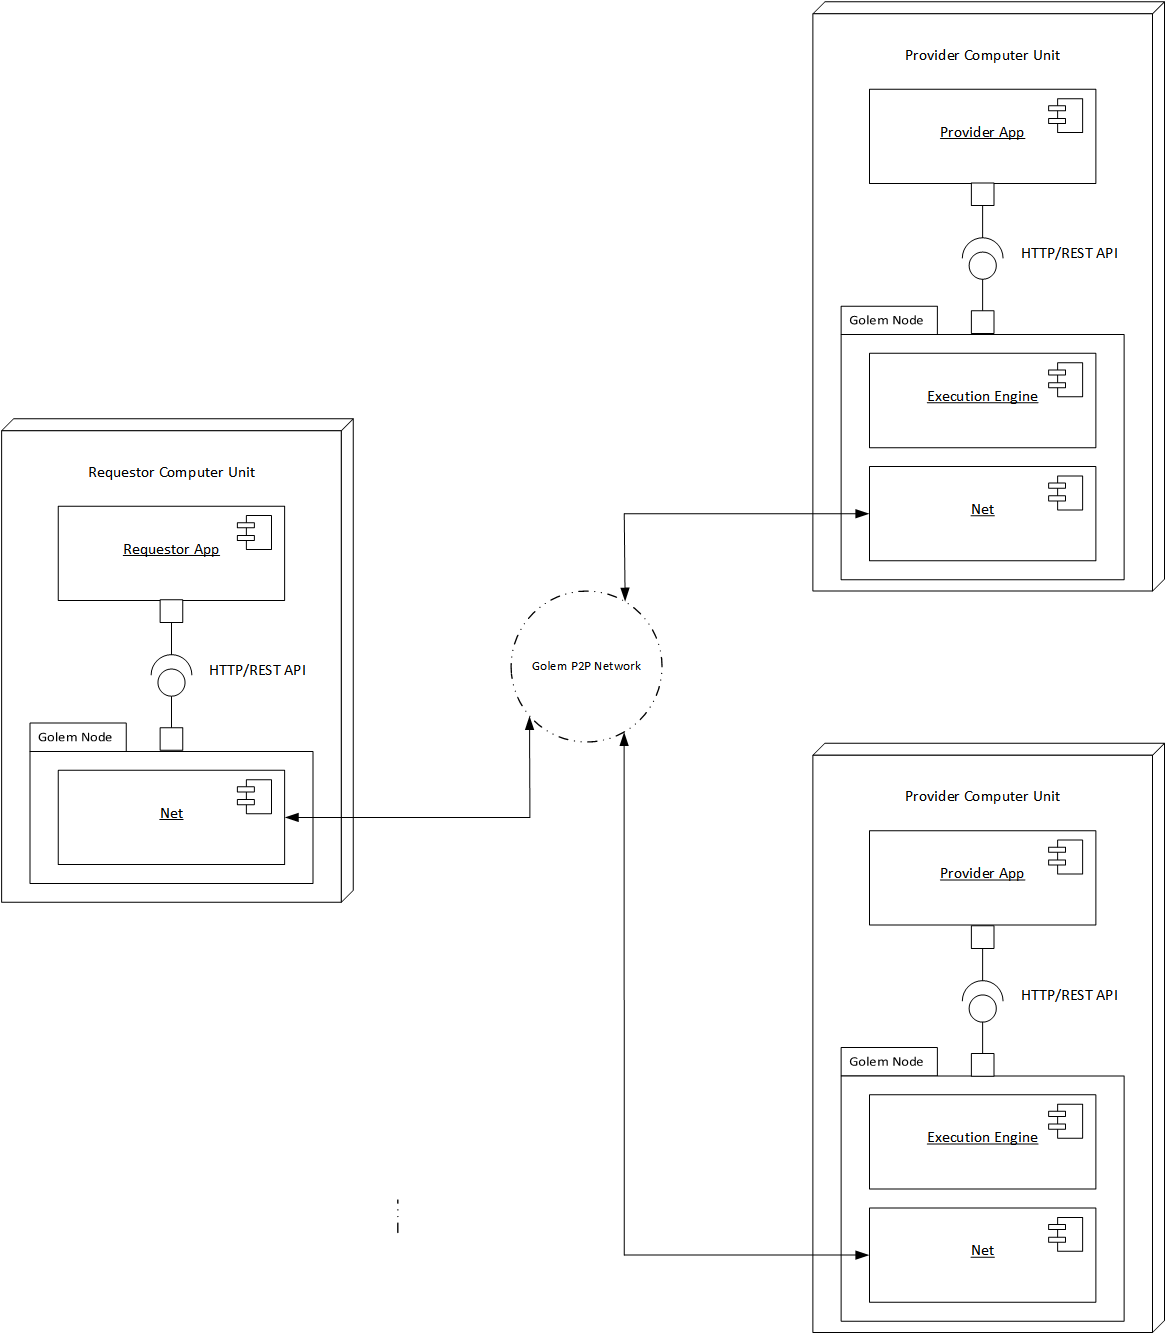
\includegraphics[width=12cm,angle=0]{./diag/Abstract/BasicDeployment-Abstract.png}
    \caption{Basic Deployment Concept}
	\label{fig:BDC}
\end{figure}

\begin{enumerate}

\item Golem Node

This is a P2P network node equipped with a unique address, which is the Golem identifier.
Golem Node is a set of generic basic services used for trading computational resources along with their API.

\item Golem Node Agent

This is a component (application) using the Golem Node API, depending on the role in the process of trading computational resources.
The basic roles in the trading process are

\begin{itemize}

\item Provider

This is an application that determines the Golem Node to the role of a seller and provider of computational resources.

\item Requestor

This is an application that determines the Golem Node to be a buyer and user of the ordered computing resources.

\end{itemize}

The basic roles of the application allow for their generic expansion, for example to the role of a Broker,
i.e. a wholesale intermediary for the sale and provision of computing resources.

\item Execution Engine

This is a component responsible for the execution of the order for computing power.

\end{enumerate}

Golem Nodes create a hybrid P2P network of distributed components with a complex communication protocol.
(Please see Figure ~\ref{fig:BPC} on page ~\pageref{fig:BPC}).

\begin{figure}[H]
    \centering
    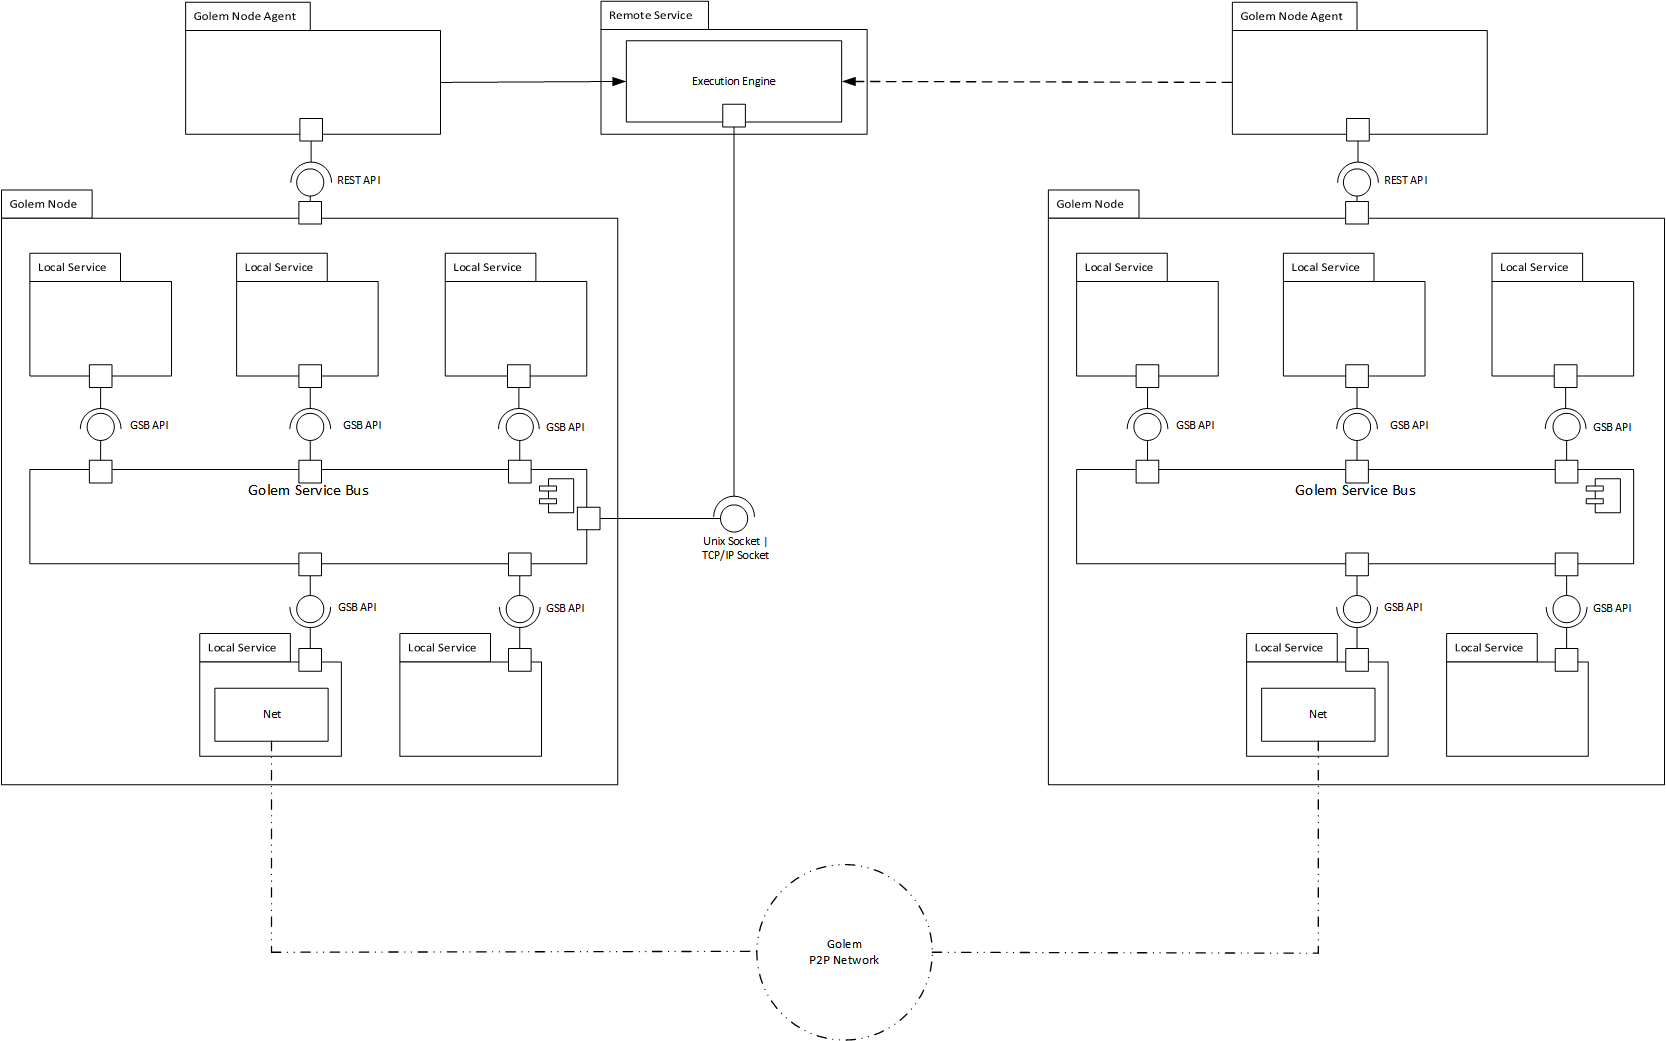
\includegraphics[width=18cm,angle=0]{./diag/Abstract/BasicPackages-Abstract.png}
	\caption{Basic Packages Concept}
    \label{fig:BPC}
\end{figure}

\newpage

A typical component consists of (Please see Figure ~\ref{fig:DPC} on page ~\pageref{fig:DPC})

\begin{figure}[H]
    \centering
    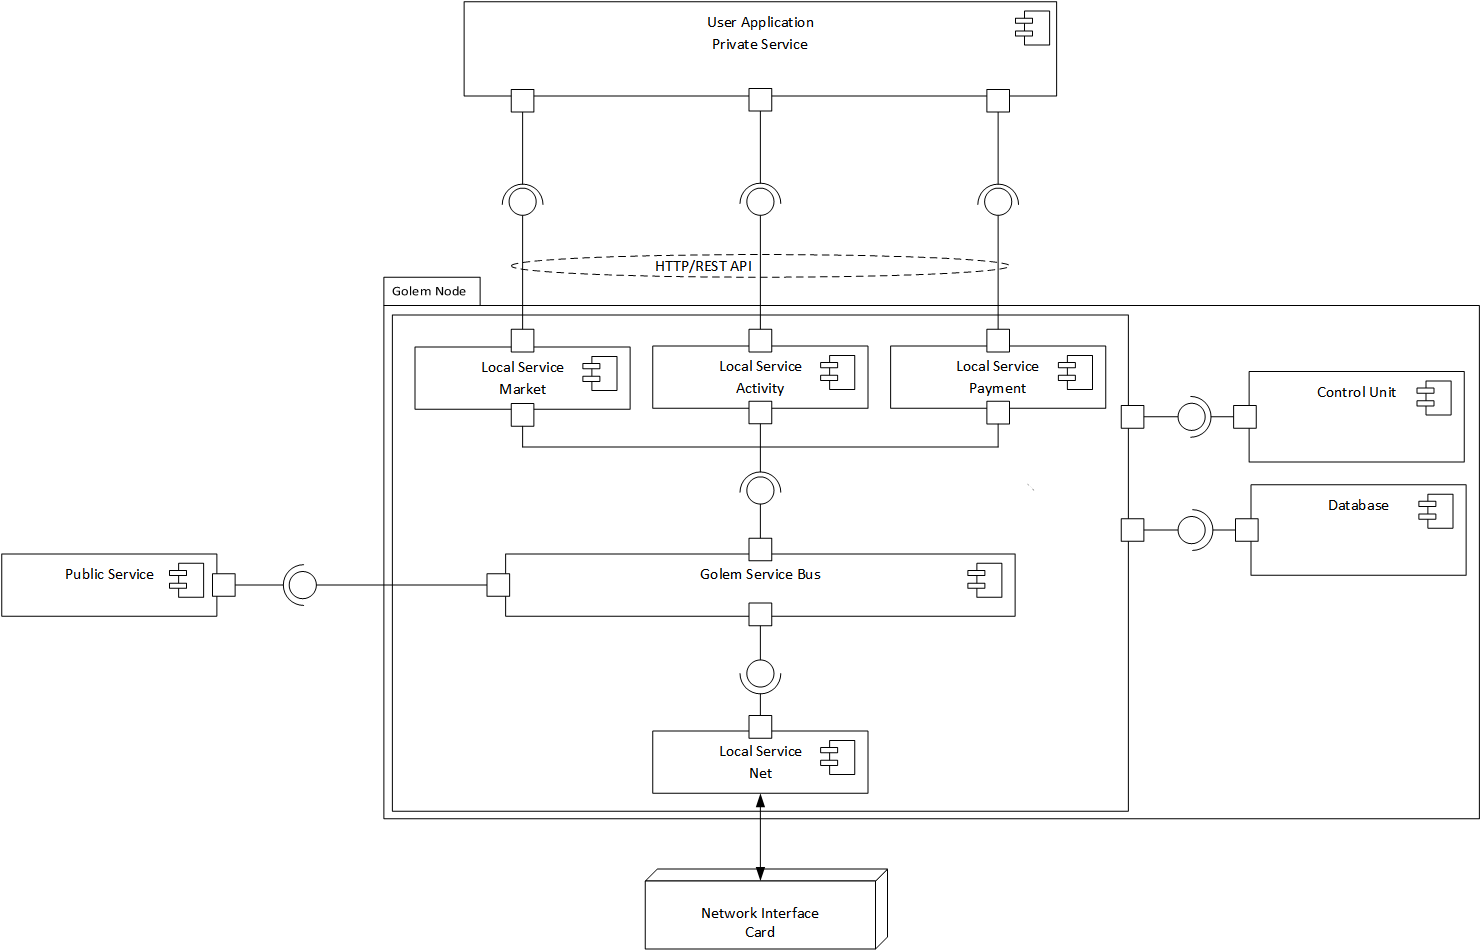
\includegraphics[width=18cm,angle=0]{./diag/Abstract/DetailPackage-Abstract.png}
	\caption{Detail Packages Concept}
    \label{fig:DPC}
\end{figure}

\begin{enumerate}

\item REST API Gateway

\item Local Services

These are the basic generic services available within the Golem Node.
They are distributed on the service bus (Golem Service Bus):

\begin{itemize}

\item Market Service

\item Activity Service

\item Payment Service

\item Identity Service

\item Net Service

This is a service necessary for communication between Golem Node nodes using P2P protocols.
It is an autonomous service, independent and isolated from other services.
More information is described later in the document

\end{itemize}

\item Remote Services

These are services available from other Golem Node nodes. These are services that allow remote launch of
applications and services that use the computing resources of Provider nodes.

This is usually the Execution Engine component.

\item Public Services

These are services that use other networks.

These are usually services that allow them to be used by other Operators, e.g. payment settlements.

\item Console

Command Line Interface (CLI) used to configure and monitor a local service within a node.

\item Database

Embeded Database is used to collect necessary data within a local service

\end{enumerate}

The subject of the trade (purchase-sale of the service of using computing resources)
is described using the service model description language (Golem SMDL).
This language is based on a simple definition of resource parameters (the list is available) and their constraints, which are expressed using filters.
The filter syntax is based on the LDAP filter syntax.

The general description of the service should include:

\begin{itemize}
\item {\bf Resource vector R} describes the infrastructure environment using qualitative and quantitative parameters as a service being traded
\item {\bf Usage vector B} defines the factors influencing the measurement of the consumption of the service of using computing resources. These factors are expressed in arbitrary counters
\item {\bf Context vector C} includes important factors that affect the price
\item {\bf Pricing function} indicates the service parameters and cumulative usage counters that affect the cost of the service
\end{itemize}

The following parties participate in the trading process

\begin{itemize}
\item {\bf requestor :} a role of a P2P network node that wants to use the computing resources of other nodes.
\item {\bf provider :} a role of a P2P network node that wants to sell its resources to other nodes
\item {\bf user :} an end user who represents the requestor node and/or the provider
\item {\bf developer :} an application developer
\end{itemize}

A user as a provider prepares an offer in the form of an Offer object using the service model description language.
A user as a requestor prepares a demand in the form of a Demand object using the service model description language.
Both the Offer and Demand objects consist of two elements:

\begin{itemize}
\item properties
\item constraints
\end{itemize}

The formal language of resource description and settlement conditions is intended to automatically or semi-automatically associate demands with offers.
The specification of the service model description language is presented later in the document.

\newpage

%A single aspect of a resource and/or service defines a dimension of the namespace.
% Thus, a set of dimensions creates a multidimensional structure of the namespace.
%Golem Agent contains basic tools for creating a decentralized market of distributed applications and services. These are:
%\begin{enumerate}
%\item {\bf Golem Market Service (GMS)}
%\item {\bf Golem Activity Service (GAS)}
%\item {\bf Golem Payment Service (GPS)}
%\item {\bf Golem Net Service (GNS)
%\item {\bf Golem Services API}
%The following APIs are available:
%\begin{itemize}
%\item Golem Market Service API (GMS API)
%\item Golem Activity Service API (GAS API)
%\item Golem Payment Service API (GPS API)
%\item Golem Net Service API (GNS API)
%\item Golem Service Bus API (GSB API)
%\end{itemize}
%All of the above services have APIs that allow you to create new decentralized and distributed applications and services,
%which use the created Golem network infrastructure (Gntw) and the genericity properties of the underlying services.
%The APIs of individual services also allow you to create interaction automation, e.g. settlements, 
%and offer optimization and orders, and many other tools.
%\end{enumerate}

%\break

%\subsection{Reference Architecture}